\section{The RationalGRL Framework}
\label{sect:overview}

In this section we present our RationalGRL framework, which allows stakeholders to discuss, analyse and argue about goal models. 

The RationalGRL framework includes two main parts: Argumentation and GRL goal modeling. The GRL part of RationalGRL allows for the creation of GRL goal models by analyzing the non-functional requirements in the requirements specification document and by refining the high-level goals into operationalized tasks. For the argumentation part, arguments and counterarguments can be put forward about various parts of this goal model. These two parts, GRL and argumentation, are developed iteratively and each side can impact the other side so that the models can be refined or new critical questions and argument schemes can be instantiated. For example, answering a critical question \emph{Is the task \texttt{A} possible?} can result in removing or adding a task in the GRL model. Similarly,  if, for example, we add a new intentional element to the GRL model, it can lead to a new critical question relevant to this intentional element and its relationships.  

Figure~\ref{fig:rationalgrl-framework} presents an overview of RationalGRL framework. At the bottom there are two activities: \emph{practical reasoning \& argumentation} and \emph{goal model construction}. As already explained, these two activities influence each other: adding elements to a goal model gives rise to new critical questions about these elements, and answering critical questions with arguments may add or delete elements from the GRL model. The activities thus provide two models: a RationalGRL argumentation model (left-hand side), which includes arguments for and against goal model elements, and a GRL goal model (right-hand side). The two types of models are connected by traceability links. In this way, it becomes possible to trace a goal model back to the original argumentative discussion about goals, tasks and requirements.

\begin{figure}[t]
\centering
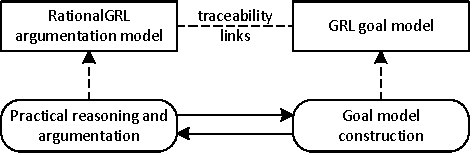
\includegraphics[width=\columnwidth]{img/framework.pdf}
\caption{The RationalGRL Framework}
\label{fig:rationalgrl-framework}
\end{figure}

In the rest of this section, we discuss the individual parts of the GRL framework. First we discuss the argument schemes and critical questions that form the basis of our framework (Section~\ref{sect:overview:as}. After this, we explain the RationalGRL language and metamodel (Section~\ref{sect:metamodel}). \todo{F}{all}{finish once paper done}

\subsection{RationalGRL: Argument Schemes and Critical Questions}
\label{sect:overview:as}

\begin{table*}[t]
\centering
\begin{tabularx}{\textwidth}{|l|l|l|X|l|l|}
\hline
\multicolumn{2}{|c|}{\textbf{Argument scheme}} & \multicolumn{2}{c|}{\textbf{Critical Questions}} & \textbf{Effect}\\
\hline
AS0 & $a$ is an actor & CQ0 & Is the actor relevant? & DISABLE\\
\hline
AS1 & Actor $a$ has resource $R$ & CQ1 &Is the resource available? & DISABLE\\
\hline
AS2 & Actor $a$ can perform task $T$ & CQ2a &Is the task possible? & DISABLE\\
&& CQ2b & Does the task contribute negatively to some softgoal? & DISABLE\\
\hline
AS3 & Actor $a$ has goal $G$ & CQ3 & Can the desired goal be realized? & DISABLE\\
\hline
AS4 & Actor $a$ has softgoal $S$ & CQ4 & Is the softgoal a legitimate softgoal?& DISABLE\\
\hline
\hline
AS5 & Goal $G$ decomposes into tasks $T_1,\ldots,T_n$ & CQ5a & Does the goal decompose into the tasks?& DISABLE\\
& & CQ5b & Does the goal decompose into any other tasks?& REPLACE\\
\hline
AS6 & Task $T$ contributes (negatively) to softgoal $S$& CQ6a & Does the task contribute to the softgoal?& DISABLE\\
&& CQ6b & Are there alternative ways of contributing to the same softgoal?& INTRO \\
&& CQ6c & Does the task contribute (negatively) to some other softgoal?& INTRO\\
\hline
AS7 & Goal $G$ contributes to softgoal $S$ & CQ7a & Does the goal contribute to the softgoal?& DISABLE\\
&& CQ7b & Does the goal contribute to some other softgoal?& INTRO\\
\hline
AS8 & Resource $R$ contributes to task $T$ & CQ8 & Is the resource required in order to perform the task?& DISABLE\\
\hline
AS9 & Actor $a$ depends on actor $b$ & CQ9 & Does the actor depend on any actors?& INTRO\\
\hline
AS10 & Task $T_1$ decomposes into tasks $T_2,\ldots,T_n$ & CQ10a & Does the task decompose into other tasks?& REPLACE\\
 &  & CQ10b & Is the decomposition type correct? (AND/OR/XOR)& REPLACE\\
\hline
AS11 & Element $IE$ is relevant & CQ11 & Is the element relevant/useful? & DISABLE\\
\hline
AS12 & Element $IE$ has name $n$ & CQ12 & Is the name clear/unambiguous? & REPLACE\\
\hline
\hline
- & - & Att & Generic counterargument & ATTACK\\
\hline
\end{tabularx}
\caption{List of argument schemes (AS0-AS13), critical questions (CQ0-CQ12), and the effect of answering them (right column).}
\label{table:argument-schemes}
\end{table*}

A core aspect of the RationalGRL framework are the argument schemes that allow us to talk about the goal models. Recall from section \ref{sect:gmas} that we ended up with a list of argument schemes and critical questions that were found in the transcripts (Table~\ref{table:transcripts:results:argumentschemes}). Using this list as a basis, we further refined our set of argument schemes and critical questions for RationalGRL into the list shown in Table~\ref{table:argument-schemes}. Note that this list of argument schemes and critical questions is not exhaustive. It is an initial list that we have obtained by coding transcripts. However, our framework is fully extensible, meaning that new argument schemes and critical questions can be added depending on the problem domain.

Schemes AS0-AS4 and AS12-AS13 are arguments for an element of a goal model, and AS5-AS11 are related to links in a goal model. The last scheme (Att) is a scheme for a generic counterargument against any type of argument that has been put forward. The critical questions presented in Table~\ref{table:argument-schemes} are related to their respective argument schemes. As was already discussed at the end of Section~\ref{sect:gmas}, answering a critical question in a certain way can have three different effects on the original argument and the corresponding GRL element:

\begin{itemize} 
\item \textsf{INTRO}: Introduce a new goal element or relationship with a corresponding argument. This operation does not attack the original argument to which the question pertains, but rather creates a new argument. %In Figure~\ref{fig:transcripts:grl}, each GRL element can be seen as the instantiation of an argument scheme. For instance, the XOR-decomposition from ``Generate Cars'' is an instantiation of AS5 as follows: ``Goal \texttt{Generate cars} XOR-decomposes into tasks \texttt{Keep same cars} and \texttt{Create new cars}''. Suppose now that the modelers that created Figure~\ref{fig:transcripts:grl} would continue their analysis by discussing critical question CQ5b: ``Does the goal \texttt{Generate cars} decompose into other tasks?'', and that they would answer this with ``Yes, namely \texttt{Choose randomly}''. This then results in the introduction of another task with the name ``Choose randomly'', and the XOR-decomposes would go from ``Generate Cars'' into the three tasks \texttt{Keep same cars}, \texttt{Create new cars}, and \texttt{Choose randomly}.'' %SG: Very good example. But should we also show it in the model as a new element?
\item \textsf{DISABLE:} Disable the element or relationship of an argument scheme to which critical questions pertains. This operation creates a new argument that disables (i.e., attacks) the original one. %In Figure~\ref{fig:transcripts:grl}, there are several examples of disabled GRL elements. The task ``Add traffic light'' (top-left in figure) is attacked by answering critical question CQ2: ``Is task Add traffic light possible?'' negatively, resulting in an argument that disables the GRL element. What we also see from Figure~\ref{fig:transcripts:grl} is that actor ``Teacher'' is disabled and thus all the elements that are bound to this actor are disabled as well. Furthermore, disabled task ``Dynamic Simulation'' also disables all incoming and outgoing links with this task.
\item \textsf{REPLACE:} Replace the element of the argument scheme with a new element. %In Figure~\ref{fig:transcripts:grl}, task ``Show map editor'' has been replaced various times, and this is shown in the figure as a \emph{refined} element. In this case, participants were discussing the correct naming for this element (CQ13), leading to various replacements of the name. While the previous names are not shown in the figure, they show up in the details pane of the corresponding element. %SG: why generate car has a star but not this one?
%\item \textsf{ATTACK:} Attack any argument with an argument that cannot be classified as a critical question. In Figure~\ref{fig:transcripts:grl}, we see one example of such a counter-attack. First, task ``Control car influx per road'' is attack by answering CQ2 (irrelevant task). However, after discussing this, participants found that this was not the case, since the problem description stated that it is important that students can control the simulation manually. Therefore, the argument that attacked the task is attacked by the counter-argument ``Important for students'', which re-enables the task ``Control car influx per road''. We provide a precise semantics for this in Section~\ref{sect:formalframework}.
\end{itemize}

%As an example of a RationalGRL model, consider Figure~\ref{fig:transcripts:grl}, which was created on the basis of transcript $t_1$. This figure shows a simplified version of the actual model in order to improve the presentation, but the full models can be found back in our repository. 

%\begin{figure*}[h!]
%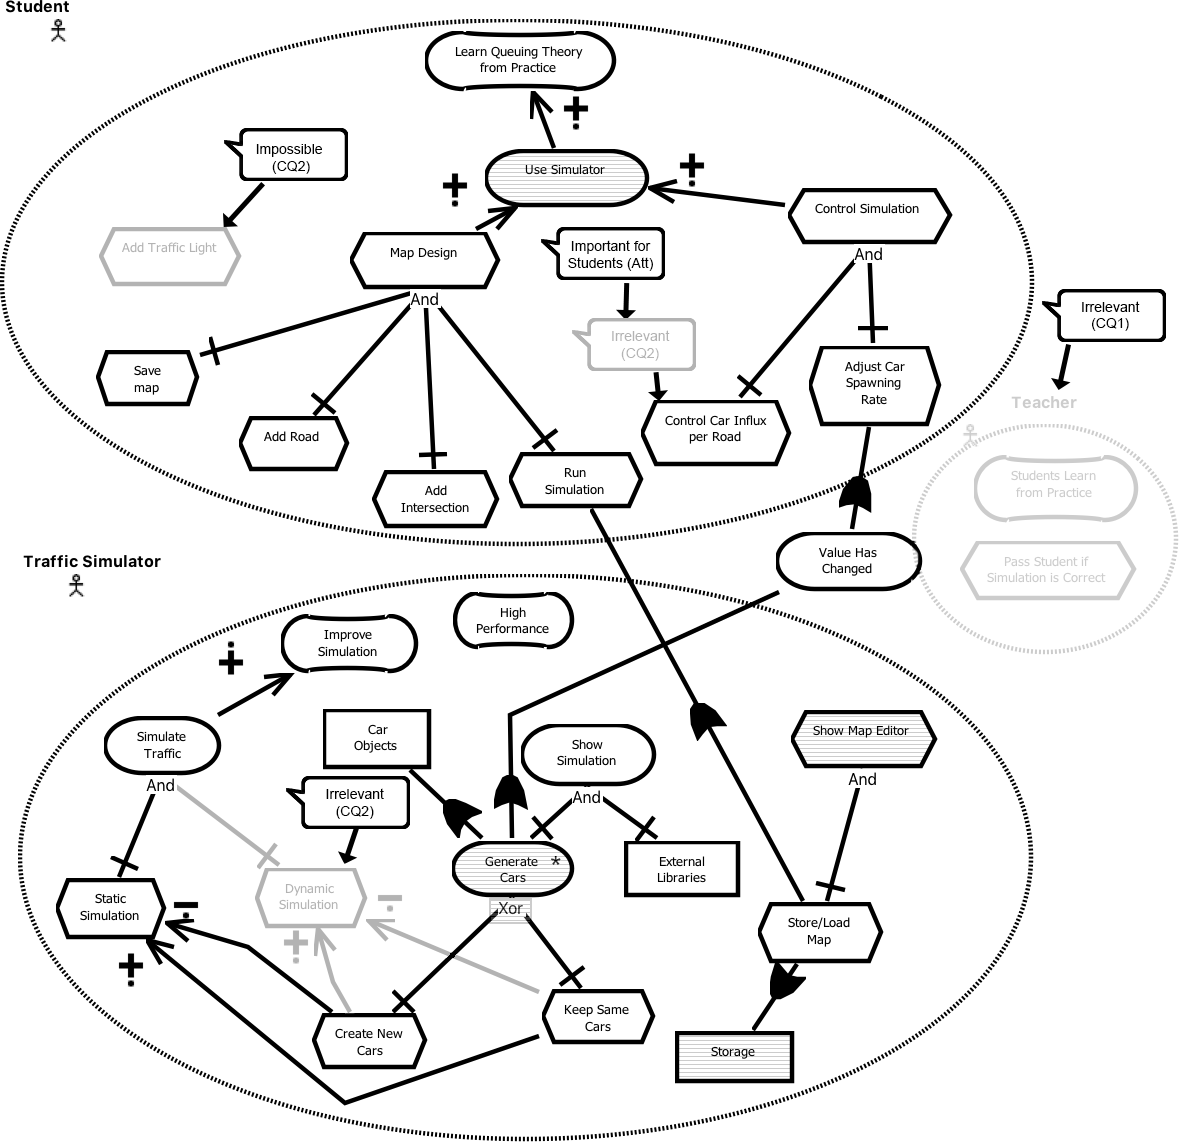
\includegraphics[width=\textwidth]{img/Fig6}
%\caption{The GRL model constructed from transcript $t_1$.} 
%\label{fig:transcripts:grl}
%\end{figure*} 

\subsection{RationalGRL: Examples from the transcripts}
Having provided the basics of the RationalGRL framework in previous sections -- Section~\ref{sect:background:grl} discusses GRL and Sections \ref{sect:background:pras} and \ref{sect:overview:as} discuss argumentation -- we now turn to some informal examples of the interactions between the argumentative discussions (i.e. the left side of the framework in Figure~\ref{fig:rationalgrl-framework}) on the one hand and GRL models (i.e. the right side of the framework in Figure~\ref{fig:rationalgrl-framework}). The formal grounding for these examples can be found in the RationalGRL Metamodel (Section~\ref{sect:metamodel}) and the logical formalization of RationalGRL (Section~\ref{sect:formalframework}).

\subsubsection{Example 1 - Introducing GRL elements through argument schemes}
In RationalGRL, each GRL element can be seen as an argument, that is, the instantiation of an argument scheme. Take the example in Figure~\ref{fig:example_AS}, which is based on the transcript excerpt shown in Table~\ref{table:transcript:decomposition}. On the left side, the arguments found in the transcript are shown, together with the argumentation scheme they are based on (cf. Table~\ref{table:argument-schemes}). The participants in the discussion argue that \emph{System} has a goal and two tasks, and that the goal AND-decomposes into the two tasks. By arguing in this way, new GRL elements are introduced (right side of Figure~\ref{fig:example_AS}). The dashed lines indicate the traceability links between the RationalGRL argumentation model on the left and the GRL model on the right. 

\begin{figure}[h]
\centering
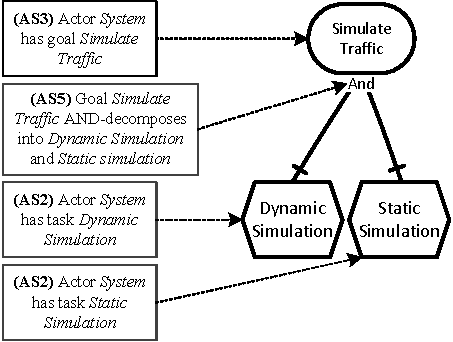
\includegraphics[width=\columnwidth]{img/fig_example_AS.pdf}
\caption{Arguments (left) and GRL elements (right). Dashed lines indicate traceability links.}
\label{fig:example_AS}
\end{figure}

\subsubsection{Example 2: Disable task \texttt{Traffic light}}

The transcript excerpt of this example is shown in Table~\ref{table:transcripts:traffic-light} in the appendix and comes from transcript $t_1$. In this example, participants sum up functionality of the traffic simulator, which are tasks that the students can perform in the simulator. All these tasks can be formalized and are instantiated from  argument scheme AS2: ``Actor \emph{Student} has tasks $T$'', where $T\in\{$Save map, Open map, Add intersection, Remove intersection, Add road, Add traffic light$\}$''. 

Once all these tasks are summed up, participant \texttt{P1} notes that the problem description states that all intersections in the traffic simulator have traffic lights, so the task \texttt{Add traffic light} is not necessary. We formalized this using the critical question CQ12: ``Is task \texttt{Add traffic light} useful/relevant?''. %TODO I think it is better to say "necessary" and "not necessary" --> change figure 8: useless --> not necessary

We visualize some of the argument schemes, critical questions, and traceability links with GRL model in Figure~\ref{fig:examples:traffic-light}. On the left side of the image, we see three of the instantiated argument schemes AS2. The bottom one, ``Actor \texttt{Student} has task \texttt{Add traffic light}'', is attacked by another argument generated from applying critical question CQ12: ``\texttt{Add traffic light} is %useless 
not necessary (\emph{All intersections have traffic lights})''. As a result, the corresponding GRL task is disabled. The other two tasks are enabled and have green traceability links.

\begin{figure}[ht!]
\centering
        \begin{tikzpicture}
        \node (a0) [argNodeIN] at (-2,0) {
        	\argtext{AS2}{Actor \emph{Student} has task \emph{Save map}}
        };
        \node (a1) [argNodeIN] at (-2,-2) {
        	\argtext{AS2}{Actor \emph{Student} has task \emph{Add road}}
        };
        \node (a2) [argNodeOUT] at (-2,-4) {
        	\argtext{AS2}{Actor \emph{Student} has task \emph{Add traffic light}}
        };
        \node (a3) [argNodeIN] at (-2,-6){
        	\argtext{}{\emph{Add traffic light} is not necessary (\emph{All intersections have traffic lights})}
        };
        \node[grl] (task1) at (2.3,0) { 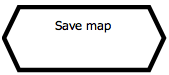
\includegraphics[scale=0.5]{img/task_save_map} };
        \node[grl] (task2) at (2.3,-2) { 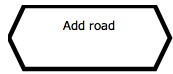
\includegraphics[scale=0.5]{img/task_add_road} };
        \node[grl, disabled] (task3) at (2.3,-4) { 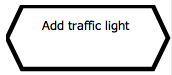
\includegraphics[scale=0.5]{img/task_add_traffic_light} };
        \node[traceNodeGREEN] (trace1a) at (-.4,-.3) {};
        \node[traceNodeGREEN] (trace1b) at (2.2,-.3) {};
        \node[traceNodeGREEN] (trace2a) at (-.4,-2.3) {};
        \node[traceNodeGREEN] (trace2b) at (2.2,-2.3) {};
        \node[traceNodeRED] (trace3a) at (-.4,-4.3) {};
        \node[traceNodeRED] (trace3b) at (2.2,-4.3) {};
         \path
    (a3) edge [attackLink] (a2)
    (a2) edge [CQLink, bend right=50] node [left,draw=none] {CQ12} (a3)
    (trace1a) edge[traceLinkGREEN] (trace1b)
    (trace2a) edge[traceLinkGREEN] (trace2b)
    (trace3a) edge[traceLinkRED] (trace3b);
\end{tikzpicture}
\caption{Argument Schemes and Critical Questions (left), GRL Model (right), and Traceability Link (dotted lines) for the Traffic Light Example.}
\label{fig:examples:traffic-light}
\end{figure}


\subsubsection{Example 3: Clarify task \texttt{Road pattern}}

The transcript excerpt of the second example is shown in Table~\ref{table:transcript:task-clarification} in Appendix~\ref{sect:transcripts:excerpts} and comes from transcript $t_3$. It consists of a number of clarification steps, resulting in the task \texttt{Choose a road pattern}. 
%TODO where is this task in the model?
%MvZ: It is in Figure 9, but not in Figure 6. Figure 6 is just a single model from our transcripts, but Figure 9 comes from another transcript. Do you think it is better to take all of the examples from the same transcript? I feel that may look a bit strange since we are completely disregarding the other transcripts then.

\begin{figure}[ht!]
\centering
        \begin{tikzpicture}[->]
        \node (a0) [argNodeOUT] at (-2,0) {
        	\argtext{AS2}{Actor \emph{Student} has task \emph{Create road}}
        };
        \node (a1) [argNodeOUT] at (-2,-2) {
        	\argtext{AS2}{Actor \emph{Student} has task \emph{Choose a pattern}}
        };
        \node (a2) [argNodeOUT] at (-2,-4.2) {
        	\argtext{AS2}{Actor \emph{Student} has task \emph{Choose a pattern preference}}
        };
        \node (a3) [argNodeIN] at (-2,-6.7) {
        	\argtext{AS2}{Actor \emph{Student} has task \emph{Choose a road pattern}}
        };
        \node[grl] (actor) at (2.3,-4) { 
        	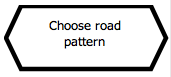
\includegraphics[scale=0.5]{img/task_choose_road_pattern} 
        };
        \node[traceNodeGREEN] (trace1) at (-.5,-7.1) {};
        \node[traceNodeGREEN] (trace2) at (2.2,-4.4) {};

\begin{pgfonlayer}{background}
         \path
    (a1) edge[attackLink] (a0)
    (a2) edge[attackLink] (a1)
    (a2) edge[attackLink, bend right=20] (a0)
    (a3) edge[attackLink] (a2)
    (a3) edge[attackLink, bend right=20] (a1)
    (a3) edge[attackLink, bend right=40] (a0);
\end{pgfonlayer}

	\path
	(a0) edge [CQLink, bend right=50] node [left,draw=none] {CQ12a} (a1)
    (a1) edge [CQLink, bend right=50] node [left,draw=none] {CQ12a} (a2)
    (a2) edge [CQLink, bend right=50] node [left,draw=none] {CQ12a} (a3)
    (trace1) edge[traceLinkGREEN] (trace2);
\end{tikzpicture}
\caption{Argument Schemes and Critical Questions (left), GRL Model (right), and Traceability Link (dotted line) for the Road Pattern Example.}
\label{fig:examples:clarification}
\end{figure}

The formalized argument schemes and critical questions are shown in Figure~\ref{fig:examples:clarification}. The discussion starts with the first instantiation of argument scheme AS2: ``Actor \texttt{Student} has task \texttt{Create road}''. 
%TODO I don't see it in Figure 6.
%MvZ: see previous comment, Figure 9 is not part of Figure 6
This argument is then challenged with critical question CQ12: ``Is the task \texttt{Create road} clear?''. Answering this question results in a new instantiation of argument scheme AS2: ``Actor \texttt{Student} has task \texttt{Choose a pattern}''. %TODO same %MvZ same
This process is repeated two more times, resulting in the final argument ``Actor \texttt{Student} has task \texttt{Choose a road pattern}''. This final argument is "un-attacked" and has a corresponding intentional element (right image). 

What is clearly shown in this example is that a clarifying argument attacks all arguments previously used to describe the element. For instance, the final argument on the bottom of Figure~\ref{fig:examples:clarification} attacks all three other arguments for a name of the element. If this is not the case, then it may occur that a previous argument is \emph{re-instantiated}, meaning that it becomes accepted again because the argument attacking it, is itself attacked. Suppose for instance that the bottom argument ``Actor \texttt{Student} has task \texttt{Choose a pattern preference}'' did not attack the second argument: ``Action \texttt{Student} has task \texttt{Choose a pattern}''. In that case, this argument would be re-instantiated, because its only attacker ``Actor \texttt{Student} has task \texttt{Choose a pattern preference}'' is itself defeated by the bottom argument. %TODO check these tasks with the GRL model of Figure 6. Also, I recommend to have the changed full  GRL model after we finish the examples to show how the model improves. 

\subsubsection{Example 4: Decompose goal \texttt{Simulate}} %TODO In fig 1, the goal is called simulate traffic which makes more sense. goal "simulate" is a bit meaningless. I suggest to update fig 6 and all the other ones accordingly. Also, we are refering to this example in example 1. Why can't we merge them?

\todo{Marc}{all}{Check whether the text matches the figure here}
The transcript excerpt of this example is shown in Table~\ref{table:transcript:decomposition} in the appendix and comes from transcript $t_3$. It consists of a discussion about the type of decomposition relationship for the goal \texttt{Simulate}.

\begin{figure}[ht]
\begin{adjustwidth}{-3em}{}
        \begin{tikzpicture}[->]
        \node (a0) [argNodeIN] at (-2,0.5) {
        	\argtext{CQ3}{Task \emph{Dynamic simulation} is not relevant}
        };
        \node (a1) [argNodeIN] at (-2,-1.5) {
        	\argtext{AS2}{Actor \emph{System} has task \emph{Dynamic simulation}}
        };
        \node (a2) [argNodeIN] at (-2,-3) {
        	\argtext{AS2}{Actor \emph{System} has task \emph{Static simulation}}
        };
        \node (a3) [argNodeOUT] at (-2,-4.5) {
        	\argtext{AS5}{Goal \emph{Simulate} AND-decomposes into \emph{Static simulation} and \emph{Dynamic simulation}}
        };
        \node (a4) [argNodeIN] at (-2,-7.5) {
        	\argtext{AS5}{Goal \emph{Simulate} OR-decomposes into \emph{Static simulation} and \emph{Dynamic simulation}}
        };
        \node[grl] (actor) at (2.2,-4) { 
        	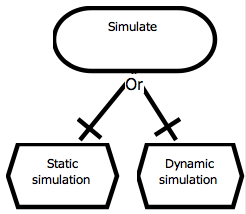
\includegraphics[scale=0.5]{img/simulate_decomposition} 
        };
        \node[traceNodeRED] (trace2a) at (-.4,-1.8) {};
        \node[traceNodeRED] (trace2b) at (3.2,-5.6) {};
        \node[traceNodeGREEN] (trace3a) at (-.4,-3.3) {};
        \node[traceNodeGREEN] (trace3b) at (1,-5.6) {};
        \node[traceNodeGREEN] (trace4a) at (-.4,-8.2) {};
        \node[traceNodeGREEN] (trace4b) at (2.2,-3.9) {};

\begin{pgfonlayer}{background}
         \path
    (a1) edge[attackLink] (a0)
    (a4) edge[attackLink] (a3);
\end{pgfonlayer}

	\path
	(a3) edge [CQLink, bend right=50] node [left,draw=none] {CQ10b} (a4)
	(a1) edge [CQLink, bend right=50] node [right,draw=none] {CQ3} (a0)
    (trace2a) edge[traceLinkRED] (trace2b)
    (trace3a) edge[traceLinkGREEN] (trace3b)
    (trace4a) edge[traceLinkGREEN, bend right] (trace4b);
\end{tikzpicture}
\end{adjustwidth}
\caption{Argument Schemes and Critical Questions (left), GRL Model (right), and Traceability Link (dotted line) of the example.} %TODO which example? 
\label{fig:examples:decomposition}
\end{figure}

The visualization of this discussion is shown in Figure~\ref{fig:examples:decomposition}. Each GRL element on the right has a corresponding argument on the left. Moreover, the original argument for an AND-decomposition is attacked by the argument for the OR-decomposition, and the new argument is linked to the decomposition relation in the GRL model. %TODO I think we can merge this easily with example 1. 

\subsubsection{Example 5: Reinstate actor \texttt{Development team}}

The transcript excerpt of this example is shown in Table~\ref{table:transcript:irrelevant-actor} in the appendix and comes from transcript $t_3$. It consists of two parts: first participant \texttt{P1} puts forth the suggestion to include actor \texttt{Development team} in the model. This is, then, questioned by participant \texttt{P2}, who argues that the professor will develop the software, so there will not be any development team. However, in the second part, participant \texttt{P2} argue that the development team should be considered, since the professor does not develop the software.

\begin{figure}[ht!]
\centering
        \begin{tikzpicture}
        \node (a0) [argNodeOUT] at (-2,0) {
        	\argtext{AS0}{Development team is relevant}
        } ;
        \node (a1) [argNodeIN] at (-2,-2.5){
        	\argtext{}{Development team is not relevant (\emph{The professor makes the software})}
        };
        \node[grl, disabled] (actor) at (2.3,-1) { 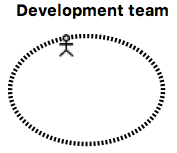
\includegraphics[scale=0.5]{img/actor_development_team} };
        \node[traceNodeRED] (trace1) at (-.5,-.3) {};
        \node[traceNodeRED] (trace2) at (2.2,-0.1) {};

         \path
    (a1) edge[attackLink] (a0)
    (a0) edge [CQLink, bend right=50] node [left,draw=none] {CQ0} (a1)
    (trace1) edge[traceLinkRED] (trace2);
\end{tikzpicture}
\caption{Argument schemes and critical questions (left), GRL model (right), and traceability link (dotted line) of a discussion about the relevance of actor Development team.}
\label{fig:examples:relevant-actor}
\end{figure}

We formalize this using a \emph{generic counterargument}, attacking the critical question. The first part of the discussion is shown in Figure~\ref{fig:examples:relevant-actor}. We formalize the first statement as an instantiation of argument scheme AS0: ``Actor \texttt{development team} is relevant''. This argument is, then, attacked by answering critical question CQ0: ``Is actor \texttt{development team} relevant? with \emph{No}. This results in two arguments, AS0 and CQ0, where CQ0 attacks AS0.'' This is shown in Figure~\ref{fig:examples:relevant-actor}, left image.

\begin{figure}[ht!]
\centering
        \begin{tikzpicture}
        \node (a0) [argNodeIN] at (-2,0) {
        	\argtext{AS0}{Development team is relevant}
        };
        \node (a1) [argNodeOUT] at (-2,-2.5){
        	\argtext{}{Development team is not relevant (\emph{The professor makes the software})}
        };
        \node (a2) [argNodeIN] at (-2,-5) {
        	\argtext{}{The professor doesn't develop the software}
        } ;
        \node[grl] (actor) at (2.3,-1) { 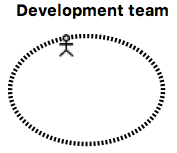
\includegraphics[scale=0.5]{img/actor_development_team} };
        \node[traceNodeGREEN] (trace1) at (-.5,-.3) {};
        \node[traceNodeGREEN] (trace2) at (2.2,-0.1) {};

         \path
    (a1) edge[attackLink] (a0)
    (a2) edge[attackLink] (a1)
    (a0) edge [CQLink, bend right=50] node [left,draw=none] {CQ0} (a1)
    (a1) edge [CQLink, bend right=50] node [left,draw=none] {Att} (a2)
    (trace1) edge[traceLinkGREEN] (trace2);
\end{tikzpicture}
\caption{Argument Schemes and Critical Questions (left), GRL Model (right), and Traceability Link (dotted line) of a Discussion about the Relevance of Actor Development Team.}
\label{fig:examples:relevant-actor2}
\end{figure}

Figure~\ref{fig:examples:relevant-actor2} shows the situation after the counter argument has been put forward. The argument ``Actor \texttt{Professor} does not develop the software'' now attacks the argument ``\texttt{Development team} is not relevant (\emph{The professor makes the software})'', which in turn attacks the original argument ``\texttt{Development team} is relevant''. As a result, the first argument is re-instantiated, which causes the actor in the GRL model to be enabled again.

\subsection{RationalGRL Metamodel}
\label{sect:metamodel}

Figure~\ref{fig:metamodel} depicts the RationalGRL metamodel linking the main elements of our argumentation extension to the main GRL elements. We describe the metamodel bottom-up, starting with the GRL package.\todo{F}{all}{Fig. 6 is now far removed from where it is mentioned in the text, we should fix this when paper is nearly finished}

The GRL package of our metamodel consists of the core GRL concepts, which constitute a part of the URN metamodel from Recommendation Z.151~\cite{URN}. These concepts represent the abstract grammar of the language, independently of the notation. This metamodel also further defines the GRL concepts and constructs introduced earlier\footnote{Note that for readability, some GRL concepts, such as contribution strength, have been omitted from the figure.}.

The GRL specification consists of \textsf{GRLModelElements}, which can be either \textsf{GRLLinkableElements} or \textsf{ElementLinks}. A \textsf{GRLLinkableElement} can again be specialized into an \textsf{Actor} or an \textsf{IntentionalElement} (which is either a \textsf{Softgoal}, \textsf{Goal}, \textsf{Task}, \textsf{Resource}, or a \textsf{Belief}). Intentional elements can be part of an actor, and \textsf{GRLLinkableElements} are connected through \textsf{ElementLinks} of different types (i.e., \textsf{Contribution, Decomposition}, or \textsf{Dependency}). Note that actors can be connected through links as well, which is done with \textsf{Dependency} links. 

The Argumentation package depicts the concepts we introduced in the previous sections. An \textsf{ArgumentScheme} represents an (uninstantiated) scheme containing variables that can be replaced with intentional elements. \textsf{CriticalQuestions} are possible ways to attack or elaborate an argument scheme. As such, each critical question applies to exactly one scheme, but each scheme can be elaborated or attacked through multiple critical questions. When an argument scheme is instantiated, we obtain an \textsf{Argument}. Therefore, each argument is associated with exactly one scheme, but a scheme can be instantiated in multiple ways. When a critical question is answered, we obtain an \textsf{AttackLink}. Each \textsf{AttackLink} is associated with at most one critical question, but a critical question can be used to attack multiple arguments. Note that an \textsf{AttackLink} can also be associated with no critical questions. This allows the user to create attacks between arguments, which do not necessarily correspond to one of the critical questions. A \textsf{RationalGRLmodel} is composed out of arguments and attack relations.

\begin{figure*}[t]
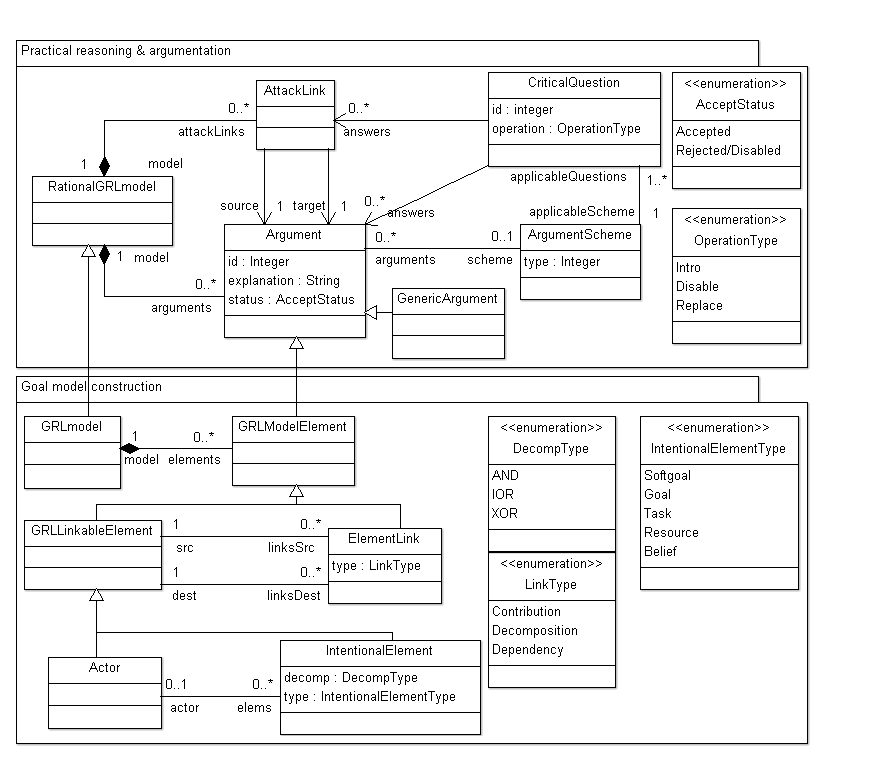
\includegraphics[width=\textwidth]{metamodel/metamodel}
\caption{The RationalGRL metamodel \todo{F}{M}{Change RationalGRLDiagram to RationalGRLmodel}}
\label{fig:metamodel}
\end{figure*}

There is only one link between the \textsf{GRL} package and the \textsf{Argumentation} package, but it is a very important one. The link specifies that each \textsf{GRLModelElement} is in fact an argument. This means that each model element inherits the \textsf{AcceptStatus} as well, allowing GRL elements to be accepted or rejected. This, furthermore, means that argument schemes can be applied to all GRL elements, capturing the intuition that each GRL element can be regarded as an instantiated argument scheme. Note that besides arguments about elements of the GRL model, we also have a \textsf{GenericArgument} which is simply a counter-argument to an existing argument that does not relate to any of the GRL elements, but can come from an external source, for instance a piece of evidence or an expert opinion. We will see various examples of such arguments in the next sections.


%I wasn't really sure what to do with the below section, so I commented it out. 
\iffalse%%%%%%%%%%%%%%%%%%%%%%%%%%%%%%%%%%%%%%%%%%%%%%%%%%%%%%%%%%%%%%%%%%%%%%%%%%%%%%
\subsection{RationalGRL Language}
The RationalGRL language is an extension of GRL, which means that it includes all the GRL elements shown in Figure~\ref{fig:grl_legend}. However, there are also new elements (Figure~\ref{fig:rationalgrllegend}):

\begin{itemize}
\item \emph{Argument}: This represents an argument that does not correspond to a GRL element. created by answering one of the critical questions which disables a GRL element, or counter-attacks a previous argument. 
\item \emph{Rejected GRL element}: If an argument or GRL element is attacked by an argument, which itself is not attacked, then this GRL element will be rejected, meaning that it does not play a role in the analysis of the GRL model. The status of arguments and 
\item \emph{Refined GRL Element}: Not all critical questions attack a GRL element. It is also possible that a critical question \emph{replaces} an existing element (for instance, by clarifying the name of the element), or that it leads to the \emph{introduction} of a new element. In these cases, the corresponding GRL element is shown with a striped background. \todo{F}{S,M}{Disabled and Refined GRL elements are not in the metamodel}
\item \emph{Attack Link}: An attack link can occur between an argument and a GRL element, or between two elements. It means that the source argument or element attacks the target argument or element.
\end{itemize} 

\begin{figure}[h]
\centering
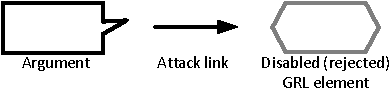
\includegraphics[width=0.35\textwidth]{img/legend}
\caption{The new elements and link of RationalGRL}
\label{fig:rationalgrllegend}
\end{figure}
\fi%%%%%%%%%%%%%%%%%%%%%%%%%%%%%%%%%%%%%%%%%%%%%%%%%%%%%%%%%%%%%%%%%%%%%%%%%%%%%%%%%%

\subsection{RationalGRL Methodology} 

We propose the following methodology (shown in Figure~\ref{fig:rationalgrl-methodology}) to develop an instance of the RationalGRL framework. Here we assume that the initial GRL models have been created based on the requirements specification documents and the discussions of the stakeholders. The rest of the steps are as follows:

\begin{figure*}[ht]
\centering
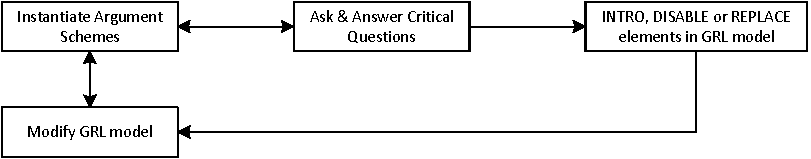
\includegraphics{img/methodology.pdf}
\caption{The RationalGRL Methodology}
\label{fig:rationalgrl-methodology}
\end{figure*}

\textbf{(1) Instantiate Argument Schemes (AS)} -- In this step, we start from the list of arguments schemes of the argumentation framework. We select an intentional element from the initial GRL model that we want to analyze and we instantiate a relevant argument scheme from the already existing list of argument schemes or by adding a new one. For example, an argument scheme can be "Goal \emph{G} contributes to softgoal \emph{S}". When an argument scheme is instantiated, it corresponds to  an argument for or against part of a goal model.

\textbf{(2) Answer Critical Questions (CQs)} -- After instantiating an argument scheme, we invoke related critical questions to attack the argument with counter-arguments.  Each argument scheme includes one or more critical questions. For example, for the argument scheme, "Goal \emph{G} contributes to softgoal \emph{S}", there are two critical questions as follows:  \emph{Does the goal contribute to the softgoal?} and \emph{Does the goal contribute to some other softgoals?}. 
%It is worth mentioning that, answering a critical question may result in a "conflict" situation. This is out of the scope of our work here.  
%MvZ: removed this sentence because I don't know what you mean with "conflict". I think We should explain it better or leave it out.
When the analyst answers  a critical question, a new argument scheme may be instantiated.  Thus, it is possible to go back and forth between this step and step (1).

\textbf{(3) Decide on Intentional Elements and their Relationships} -- By answering a critical question, one of the four following cases can occur: \textsf{INTRO}, \textsf{DISABLE}, \textsf{REPLACE} or \textsf{ATTACK}.  Any of these cases can  impact the arguments and corresponding GRL intentional elements.  \textsf{INTRO} means that 
a new argument scheme is created. That means, the current argument scheme related to the critical question does not get attacked.  In the case of \textsf{DISABLE}, the intentional element or its related links are disabled or removed from the models. \textsf{REPLACE} introduces a new argument and attacks the original argument at the same time. This means that the original element of the argument scheme is replaced with a new one. \textsf{ATTACK} is a generic counterargument which attacks any argument with another argument when new evidence occurs.  

\textbf{(4) Modify GRL Models} -- In this step, we modify the GRL models based on the situation of step (3). That is, one of the following situation can happen with respect to the initial GRL model: 1) a new intentional element or a new link is introduced; 2) an existing intentional element or an existing link gets disabled (removed) from the model; or 3) an existing intentional element or link is replaced by a new one. This results in a new modified GRL. The new GRL model can then impact the argument schemes and instantiate another argument scheme (Step (1)).   

We can continue these four steps until there is no more intentional element or link to analyze or we reach a satisfactory model. 

\subsubsection{Example 6: Methodology example}

In this section, we present a small example for the RationalGRL methodology. This example is based on the traffic simulator example described in Section~\ref{sect:goals:runningexample}. We base argument schemes and critical questions of this example on a transcript containing discussions about the development of this traffic simulator system. %These transcripts are created as part of two master theses on improving design reasoning~\cite{masterthesis1,masterthesis2}. %TODO again?
%We provide several more examples in Section~\ref{sect:examples}.

As mentioned in Section~\ref{sect:goals:runningexample}, a group of stakeholders are developing a goal model for a traffic simulator example and they are modeling the goal \texttt{Simulate Traffic} using the RationalGRL methodology. This proceeds in the following way:
\begin{itemize}
\item
First they start %at step \emph{Modify GRL models} (Figure~\ref{fig:rationalgrl-methodology}), 
with the initial GRL model (Figure~\ref{fig:example-small}) and they invoke the intentional element \texttt{Simulate Traffic}. 
\item Next, they switch to the argumentation part (step \emph{Instantiate arguments schemes}). They answer critical question \emph{Does Simulate Traffic AND-decompose into any tasks?} with \emph{Yes: namely tasks ``Dynamic Simulation'' and ``Static Simulation"}.
\item As a result, two argument schemes are created, namely:
\begin{itemize}
\item Actor \texttt{Traffic Simulator} has task \texttt{Dynamic Simulation}
\item Actor \texttt{Traffic Simulator} has task \texttt{Static Simulation}
\end{itemize}
\item In the GRL model, this corresponds to the addition of two tasks, and an AND-decomposition from the goal \emph{Simulate Traffic} to these two tasks.
\item Next, the stakeholders test the validity of their goal model by answering more critical question. They answer two critical questions:
\begin{itemize}
\item
CQ \emph{Is task ``Dynamic Simulation'' relevant} is answered with ``No, it is not relevant since the problem specification explicitly states dynamic simulations are not required''. Thus, the corresponding GRL intentional element is disabled.
\item The decomposition is changed from AND to OR, since it turned out not both tasks can be implemented together.
\end{itemize}
\end{itemize}

An excerpt of the RationalGRL model is shown in Figure~\ref{fig:examples:decomposition}. %TODO You need to update goal "simulate" in this figure to "Simulate Traffic".  Also, I don't think we should really call it the rational GRL model. it is an excerpts of the model. 